% ! TeX program = lualatex
\documentclass[a4paper,11pt]{article} 
% packages
\usepackage{censor}
\StopCensoring
\usepackage{fontspec}
\setmainfont{EB Garamond}
% for tironian et fallback
% % \directlua{luaotfload.add_fallback
% % ("emojifallback",
% %      {"Noto Serif:mode=harf"}
% % )}
% % \setmainfont{EB Garamond}[RawFeature={fallback=emojifallback}]

\setmonofont[Scale=MatchLowercase]{Deja Vu Sans Mono}
\usepackage[a4paper,left=2cm,right=2cm,top=\dimexpr15mm+1.5\baselineskip,bottom=2cm]{geometry}
\setlength{\parindent}{0pt}

\usepackage{fancyhdr}       % Headers and footers 
\fancyhead[R]{\normalfont \leftmark}
\fancyhead[L]{}
\pagestyle{fancy}

\usepackage{microtype}      % Slightly tweak font spacing for aesthetics
\usepackage[english]{babel} % Language hyphenation and typographical rules
\usepackage{xcolor}
\definecolor{linkblue}{RGB}{0, 64, 128}
\usepackage[final, colorlinks = false, urlcolor = linkblue]{hyperref} 
% \newcommand{\secref}[1]{\textbf{§~\nameref{#1}}}
\newcommand{\secref}[1]{\textbf{§\ref{#1}~\nameref{#1}}}

\usepackage[most]{tcolorbox}
\usepackage{changepage}     % adjust margins on the fly
\usepackage{amsmath,amssymb}

\usepackage{minted}
\usemintedstyle{algol_nu}

\usepackage{pgfplots}
\pgfplotsset{width=\textwidth,compat=1.9}

\usepackage{caption}
\newenvironment{code}{\captionsetup{type=listing}}{}
\captionsetup[listing]{skip=0pt}
\setlength{\abovecaptionskip}{5pt}
\setlength{\belowcaptionskip}{5pt}

\usepackage[yyyymmdd]{datetime}
\renewcommand{\dateseparator}{--}

\usepackage{enumitem}

\usepackage{titlesec}

\author{Andrew Hayes}

\begin{document}
\begin{titlepage}
    \begin{center}
        \hrule
        \vspace*{0.6cm}
        \Huge \textsc{ct421}
        \vspace*{0.6cm}
        \hrule
        \LARGE
       \vspace{0.5cm}
       Artificial Intelligence
       \vspace{0.5cm}
       \hrule

       \vfill

       \hrule
        \begin{minipage}{0.495\textwidth} 
            \vspace{0.4em}
            \raggedright
            \normalsize 
            \begin{tabular}{@{}l l}
                Name: & Andrew Hayes \\
                Student ID: & 21321503 \\
                E-mail: & \href{mailto://a.hayes18@universityofgalway.ie}{a.hayes18@universityofgalway.ie} \\
            \end{tabular}
        \end{minipage}
        \begin{minipage}{0.495\textwidth} 
            \raggedleft
            \vspace*{0.8cm}
            \Large
            \today
            \vspace*{0.6cm}
        \end{minipage}
        \medskip\hrule 
    \end{center}
\end{titlepage}

\pagenumbering{roman}
\newpage
\tableofcontents
\newpage
\setcounter{page}{1}
\pagenumbering{arabic}

\section{Introduction}
\subsection{Assessment}
\begin{itemize}
    \item   Exam: 60\%.
    \item   2 projects: 20\% each.
\end{itemize}

\subsection{Introduction to Artificial Intelligence}
The field of Artificial Intelligence has evolved \& changed many times over the years, with changes focussing both on the problems \& approaches in the field;
many problems that were considered typical AI problems are now often considered to belong in different fields.
There are also many difficulties in defining intelligence: the \textbf{Turing test} attempts to give an objective notion of intelligence and abstracts away from any notions of representation, awareness, etc.
It attempts to eliminate bias in favour of living beings by focusing solely on content of questions \& answers.
There are many criticisms of the Turing test:
\begin{itemize}
    \item   Bias towards symbolic problem-solving criticisms;
    \item   Doesn't test many aspects of human intelligence;
    \item   Possibly constrains notions of intelligence.
\end{itemize}

\subsubsection{Approaches to AI}
\begin{itemize}
    \item   \textbf{Classical AI} uses predicate calculus (\& others) and logical inference to infer or find new information.
            It is a powerful approach for many domains, but issues arise when dealing with noise or contradictory data.

    \item   \textbf{Machine learning} learns from data and uses a distributed representation of learned information.
            It is typified by neural networks \& deep learning approaches.

    \item   \textbf{Agent-based systems} view intelligence as a collective emergent behaviour from a large number of simple interacting individuals or \textit{agents}.
            Social systems provide another metaphor for intelligence in that they exhibit global behaviours that enable them to solve problems that would prove impossible for any of the individual members.
            Properties of agent-based systems / artificial life include:
            \begin{itemize}
                \item   Agents are autonomous or semi-autonomous;
                \item   Agents are situated;
                \item   Agents are interactional;
                \item   Society is structured;
                \item   Intelligence is emergent.
            \end{itemize}
\end{itemize}

\section{Search}
Many problems can be viewed as a \textbf{search} problem;
consider designing an algorithm to solve a sudoku puzzle: in every step, we are effectively searching for a move (an action) that takes us to a correct legal state.
To complete the game, we are iteratively searching for an action that brings us to legal board and so forth until completion.
Other examples include searching for a path in a maze, word ladders, chess, \& checkers.
The problem statement can be formalised as follows:
\begin{itemize}
    \item   The problem can be in various states.
    \item   We start in an initial state.
    \item   There is a set of actions available.
    \item   Each action changes the state.
    \item   Each action has an associated cost.
    \item   We want to reach some goal while minimising cost.
\end{itemize}

More formally:
\begin{itemize}
    \item   There is a set of (possible/legal) states $S$;
    \item   There is some start state $s_0 \in S$;
    \item   There is a set of actions $A$ and action rules $a(s) \rightarrow s'$;
    \item   There is some goal test $g(s) \rightarrow \{0,1\}$ that tests if we have satisfied our goal;
    \item   There is some cost function $C(s,a,s') \rightarrow \mathbb{R}$ that associates a cost with each action;
    \item   Search can be defined by the 5-tuple $(S,s,a,g,C)$.
\end{itemize}

We can then state the problem as follows:
find a sequence of actions $a_1 \dots a_n$ and corresponding states $s_0 \dots s_n$ such that:
\begin{itemize}
    \item   $s_0 = s$
    \item   $s_i = a_i(S_{i-1})$
    \item   $g(s_n) = 1$
\end{itemize}
while minimising the overall cost $\sum^n_{i=1} c(a_i)$.
\\\\
The problem of solving a sudoku puzzle can be re-stated as:
\begin{itemize}
    \item   Sudoku states: all legal sudoku boards.
    \item   Start state: a particular, partially filled-in, board.
    \item   Actions: inserting a valid number into the board.
    \item   Goal test: all cells filled with no collisions.
    \item   Cost function: 1 per move.
\end{itemize}

We can conceptualise this search as a \textbf{search tree}: a node represents a state, and the edges from a state represent the possible actions from that state, with the edge pointing to the new resulting state from the action.
Important factors of a search tree include:
\begin{itemize}
    \item   The breadth of the tree (branching factor).
    \item   The depth of the tree.
    \item   The minimum solution depth.
    \item   The size of the tree $O(b^d)$.
    \item   The \textbf{frontier:} the set of unexplored nodes that are reachable from any currently explored node.
    \item   Choosing which node to explore next is the key in search algorithms.
\end{itemize}

\subsection{Uninformed Search}
In \textbf{uninformed search}, no information is known (or used) about solutions in the tree.
Possible approaches include expanding the deepest node (depth-first search) or expanding the closest node (breadth-first search).
Properties that must be considered for uninformed search include completeness, optimality, time complexity (the total number of nodes visited), \& space complexity (the size of the frontier).

\begin{code}
\begin{minted}[linenos, breaklines, frame=single, escapeinside=||]{python}
visited = {};
frontier = {|$s_0$|};
goal_found = False;

while (not goal_found):
    node = frontier.next();
    frontier.delete(node);

    if (g(node)):
        goal_found = True;
    else
        visited.add(node);
        for child in node.children():
            if (not visited.contains(child)):
                frontier.add(child);

\end{minted}
\caption{Pseudocode for an uninformed search}
\end{code}

The manner in which we expand the node is key to how the search progresses.
The way in which we implement \mintinline{python}{frontier.next()} determines the type of search; otherwise the basic approach remains unchanged.
\\\\
\textbf{Depth-first search} is good regarding memory cost, but produces suboptimal solutions:
\begin{itemize}
    \item   Space: $O(bd)$.
    \item   Time: $O(b^d)$.
    \item   Completeness: only for finite trees.
    \item   Optimality: no.
\end{itemize}

\textbf{Breadth-first search} produces an optimal solution, but is expensive with regards to memory cost:
\begin{itemize}
    \item   Space: $O(b^{m+1})$, where $m$ is the depth of the solution in the tree.
    \item   Time: $O(b^m)$.
    \item   Completeness: yes.
    \item   Optimality: yes (assuming constant costs).
\end{itemize}

\textbf{Iterative deepening search} attempts to overcome some of the issues of both breadth-first and depth-first search.
It works by running depth-first search to a fixed depth of $z$ by starting at $d=1$ and if no solution is found, incrementing $d$ and re-running.
\begin{itemize}
    \item   Low memory requirements (equal to depth-first search).
    \item   Not many more nodes expanded than breadth-first search.
    \item   Note that the leaf level will have more nodes than the previous layers.
\end{itemize}

Thus far, we have assumed each edge has a fixed cost; consider the case where the costs are not uniform:
neither depth-first search or breadth-first search are guaranteed to find the least-cost path in the case where action costs are not uniform.
One approach is to choose the node with the lowest cost: order the nodes in the frontier by cost-so-far (cost of the path from the start state to the current node) and explore the next node with the smallest cost-so-far, which gives an optimal and complete solution (given all positive costs).

\subsection{Informed Search}
Thus far, we have assumed we know nothing about the search space; what should we do if we know \textit{something} about the search space?
We know the cost of getting to the current node: the remaining cost of finding the solution is the cost from the current node to the goal state; therefore, the total cost is the cost of getting from the start state to the current node, plus the cost of getting from the current node to the goal state.
We can use a (problem-specific) \textbf{heuristic} $h(s)$ to estimate the remaining cost: $h(s) = 0$ is $s$ is a goal.
A good heuristic is fast to compute and close to the real costs.
\\\\
Given that $g(s)$ is the cost of the path so far, the \textbf{A* algorithm} expands the node $s$ to minimise $g(s) + h(s)$.
The frontier nodes are managed as a priority queue.
If $h$ never overestimates the cost, the A* algorithm will find the optimal solution.

\subsection{Adversarial Search}
The typical game setting is as follows:
\begin{itemize}
    \item   2 player;
    \item   Alternating turns;
    \item   Zero-sum (gain for one, loss for another);
    \item   Perfect information.
\end{itemize}

A game is said to be \textbf{solved} if an optimal strategy is known.
\begin{itemize}
    \item   A \textbf{strong solved} game is one which is solved for all positions;
    \item   A \textbf{weak solved} game is one which is solved for some (start) positions.
\end{itemize}

A game has the following properties:
\begin{itemize}
    \item   A set of possible states;
    \item   A start state;
    \item   A set of actions;
    \item   A set of end states (many);
    \item   An objective function;
    \item   Control over actions alternates.
\end{itemize}

The \textbf{minimax algorithm} computes a value for each node, going backwards from the end-nodes.
The \textbf{max player} selects actions to maximise return, while the \textbf{min player} selects actions to minimise return.
The algorithm assumes perfect play from both players.
For optimal play, the agent has to evaluate the entire game tree.
Issues to consider include:
\begin{itemize}
    \item   Noise / randomness;
    \item   Efficiency -- size of the tree;
    \item   Many game trees are too deep;
    \item   Many game trees are too broad.
\end{itemize}

\textbf{Alpha-beta pruning} is a means to reduce the search space wherein sibling nodes can be pruned based on previously found values.
Alpha represents the best maximum value found so far (for the maximising player), and beta represents the best minimum value found so far (for the minimising player).
If a node's value proves irrelevant (based on the alpha \& beta values), its entire subtree can be discarded.
In reality, for many search scenarios in games, even with alpha-beta pruning, the space is much too large to get to all end states.
Instead, we use an \textbf{evaluation function} which is effectively a heuristic to estimate the value of a state (the probability of a win or a loss).
The search is ran to a fixed depth and all states are evaluated at that depth.
Look-ahead is performed from the best states to another fixed depth.
\\\\
\textbf{Horizon effects} refer to the limitations that arise when the algorithm evaluates a position based on a finite search depth (the horizon):
\begin{itemize}
    \item   What if something interesting / unusual / unexpected occurs at $\text{horizon}+1$?
    \item   How do you identify that?
    \item   When to generate and explore more nodes?
    \item   Deceptive problems.
\end{itemize}

\subsection{Monte Carlo Tree Search}
Minimax and alpha-beta pruning are both useful approaches, and alpha-beta pruning effectively results in computing the square root of the branching factor.
In many cases, however, game trees have too high a \textbf{blocking factor} and evaluating the leaf nodes is not possible; instead, an \textbf{estimation function} is used instead.
\\\\
\textbf{Monte Carlo tree search} continually estimates the value of tree nodes.
It combines ideas from classical tree search with ideas from machine learning, and balances the exploration of unseen space with exploitation of the best known move.
Monte Carlo tree search works by exploring all potential options at the time. 
The best move is identified and other option are searched for while validating how good the current action is.
It uses \textbf{play out}, which is simulation considering random actions.
\begin{enumerate}
    \item   \textbf{Selection:} pick a suitable path.
    \item   \textbf{Expansion:} expand from that path.
    \item   \textbf{Simulation:} simulation / play outs.
    \item   \textbf{Back propagation:} update states.
\end{enumerate}

There is a trade-off between exploration and exploitation; the balance is usually controlled by the number of parameters / factors, including the number of wins, simulations, \& exploration cost.
Monte Carlo grid search is used in a large number of domains, including AlphaGo, DeepMind, \& many video games.

\subsection{Local Search Algorithms}
In many domains, we are only interested in the goal state: the path to finding the goal is irrelevant.
The main idea in \textbf{local search algorithms} is to maintain the current state and repeatedly try to improve upon the current state.
This results in little memory overhead and can find reasonable solutions even in large or infinite spaces.
Local search algorithms are suitable only for certain classes of problems in which maximising (or minimising) certain criteria among a number of candidate solutions is desirable.
Local search algorithms are \textbf{incomplete algorithms}, as they may not find the optimal solution.

\subsection{Hill Climbing}
\textbf{Hill climbing} involves moving in the direction of increasing value and stopping when a peak is reached.
There is no look-ahead involved, and only the current state \& the objective function are maintained.
One problem with hill climbing algorithms is local maxima \& minima; therefore, the success of the algorithm depends on the shape of the search space.
One approach to solve this problem is \textbf{random restart}.

\begin{code}
\begin{minted}[linenos, breaklines, frame=single, escapeinside=||]{python}
current_node = initial_state;

while (stopping_criteria):
    neighbour = current_node.fittest_neighbour;

    if neighbour.value > current_node.value:
        current_node = neighbour;
\end{minted}
\caption{Hill climbing pseudocode}
\end{code}

One problem that can be solved with a hill climbing algorithm is the \textbf{8 queens problem}: place 8 queens on a chess board so that no two queens are attacking each other.
The problem can be stated more formally as: given an 8 $\times$ 8 grid, identify 8 squares so that no two squares are on the same row, column, or diagonal.
The problem can also be generalised to an $N \times N$ board.
An algorithm can be generated using hill climbing to find a solution.
However, it must be noted that the algorithm may get caught at a local maximum.
\\\\
\textbf{Simulated annealing} attempts to avoid getting stuck in local maxima by randomly moving to another state.
The move is based on the fitness of the current state, the new state, and the \textbf{temperature} (a parameter which decreases over time and reduces the probability of changing states).

\subsection{Well-Known Optimisation Problems}
\subsubsection{Knapsack Problem}
There are a set of items, each with a value \& a weight.
The goal is to select a subset of items such that the weight of these items is below a threshold and the sum of the values is optimised / maximised.
The problem is how to select those items.
More formally, given two $n$-tuples of values $< v_0, v_1, \dots, v_n>$ and $<w_0, w_1, \dots, w_n>$, choose a set of items $i$ from the $n$items such that $\sum_i v(i)$ is maximised and $\sum_iw(i) \leq T$.
\\\\
The brute force approach is to enumerate all subsets and keep the subset that gives the greatest payoff: $O(2^n)$.
The greedy approach is more efficient but won't give the best solution.
\\\\
There are many variations on the knapsack problem; the variation described above is the 0/1 knapsack problem;
there are other scenarios where part of an item may be taken, variations wherein there are constraints over the items where the value of an item is dependent on another item being chosen or not, and variations with multiple knapsacks.

\subsection{Travelling Salesman Problem}
Given $N$ cities, devise a tour that involves visiting every city once.
The distance, or \textit{cost}, between pairs of cities is known and the goal is to minimise the cost of the tour.
There are many applications of this problem in scheduling \& optimisation.
\\\\
The brute force approach is to enumerate all tours and choose the cheapest, and is computationally intractable.

\section{Genetic Algorithms}
\textbf{Genetic algorithms} are directed search algorithms inspired by biological evolution, developed by John Holland in the 1970s to study the adaptive processes occurring in natural systems.
They have been used as search mechanisms to find good solutions for a range of problems.
At a high level, the algorithm is as follows:
\begin{enumerate}
    \item   Produce an initial population of individuals.
    \item   Evaluate the fitness of all individuals.
    \item   While the termination condition is not met, do:
            \begin{enumerate}[label=\arabic*.]
                \item   Select the fitter individuals for reproduction.
                \item   Recombine between individuals.
                \item   Mutate individuals.
                \item   Evaluate the fitness of the modified individuals.
                \item   Generate a new population.
            \end{enumerate}
\end{enumerate}

There are many potential options for the representation of chromosomes, including bit strings, integers, real numbers, lists of rules/instructions, \& programs.
To initialise the population, we typically start with a population of randomly generated individuals, but we can also use a previously-saved population, a set of solutions provided by a human expert, or a set of solutions provided by another algorithm.
As rules of thumb, we generally use a data structure as close as possible to the natural representation, write appropriate genetic operators as needed, and, if possible, ensure that all genotypes correspond to feasible solutions.
Selection can be fitness-based (roulette wheel), rank-based, tournament selection, or elitism.
\\\\
\textbf{Crossover} is a vital component of genetic algorithms that allows the recombination of good sub-solutions and speeds up search early in evolution.
\textbf{Mutation} represents a change in the gene; the main purpose is to prevent the search algorithm from becoming trapped in a local maxima.
\\\\
As a simple example, suppose that one wishes to maximise the number of \verb|1|s in a string of $l$ binary digits.
Similarly, we could set the target to be an arbitrary string of \verb|1|s and \verb|0|s.
An individual can be represented as a string of binary digits.
The fitness of a candidate solution is the number of \verb|1|s in its genetic code.
A related problem, maintaining the same representation as before, is to modify the fitness function as follows:
for strings of length $l$ with $x$ \verb|1|s, if $x > 1$, then fitness is equal to $x$; else, fitness is equal to $l+k$ for $k>0$.

\subsection{Schema Theorem}
Consider a genetic algorithm using only a binary alphabet.
$\{0,1,*\}$ is the alphabet, where $*$ is a special wildcard symbol which can be either $0$ or $1$.
A \textbf{schema} is any template comprising a string of these three symbols;
for example the schema $[1*1*]$ represents the following four strings: $[1010]$, $[1011]$, $[1110]$, $[1111]$.
\\\\
The \textbf{order} of a schema $S$ is the number of fixed positions ($0$ or $1$) presented in the schema.
For example, $[01*1*]$ has order $3$, $[1*1*10*0]$ has order $5$.
The order of a schema is useful in estimating the probability of survival of a schema following a mutation.
\\\\
The \textbf{defining length} of a schema $S$ is the distance between the first and last fixed positions in the schema.
For example, the schema $S_1 = [01*1*]$ has defining length $3$.
The defining length of a schema indicates the survival probability of the schema under crossover.
\\\\
Given selection based on fitness, the expected number of individuals belonging to a schema $S$ at generation $i+1$ is equal to the number of them present at generation $i$ multiplied by their fitness over the average fitness.
An ``above average'' schema receives an exponentially increasing number of strings over the evolution.
The probability of a schema $S$ surviving crossover is dependent on the defining length: schemata with above-average fitness with short defining lengths will still be sampled at exponentially increasing rates.
The probability of a schema $S$ surviving mutation is dependent on the order of the schema: schemata with above-average fitness with low orders will still be sampled at exponentially increasing rates.
\\\\
The \textbf{schema theorem} states that short, low-order, above-average schemata receive exponentially increasing representation in subsequent generations of a genetic algorithm.
The \textbf{building-block hypothesis} states that a genetic algorithm navigates the search space through the re-arranging of short, low-order, high-performance schemata, termed \textit{building blocks}.

\subsection{Landscapes}
A \textbf{landscape} is a visualisation of the relationship between genotype \& fitness;
it can give an insight into the complexity of the problem at hand.
Landscapes can be adaptive.

\begin{figure}[H]
    \centering
    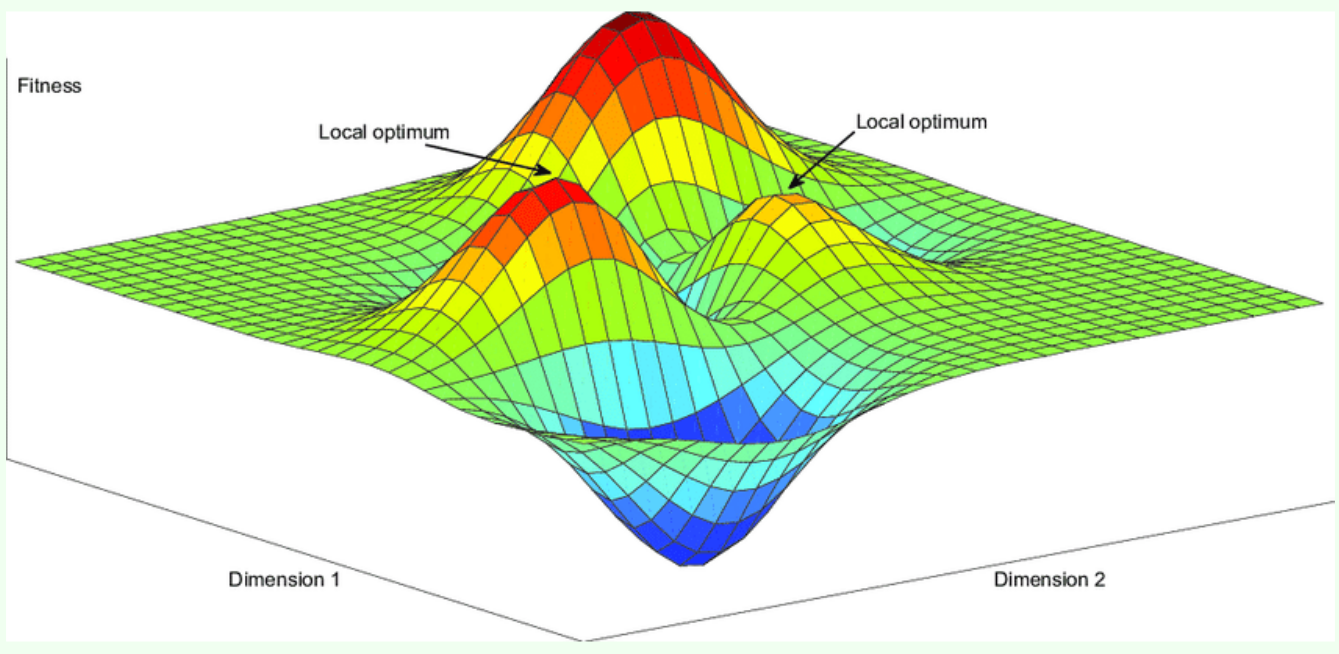
\includegraphics[width=\textwidth]{./images/landscape.png} \caption{Fitness landscape example. The peaks on the landscape represent high fitness and hence the ability of the genotype to survive. The valleys or troughs indicate low fitness.}
\end{figure}

An \textbf{NK fitness landscape} is a model of genetic interactions, developed to explain \& explore the effects of local features on the ruggedness of a fitness landscape -- \textit{ruggedness} plays a key roles in ascertaining how difficult it is to find the global optimum.
NK landscapes allow us to tune the ruggedness.
Each component (gene) of the solution space makes a contribution to the fitness;
the contribution to the landscape depends on the value of that gene itself but also on the state of $K$ other nodes, where $K$ can be changed to give different landscapes.
If $K=0$, all genes are independent and this is typically a smooth multi-modal landscape; as $K$ increases, the landscape becomes more rugged.
\\\\
One approach to create NK fitness landscapes is to use a \textit{lookup table} of size $2^K$ where each row in the lookup table represents the neighbourhood values and the fitness achieved.
Variations on NK fitness landscapes can be made by using non-uniform interaction sizes or allowing non-adjacent genes to influence each other's fitness.
\\\\
\textbf{Fitness clouds} can be created by randomly sampling the population, generating $K$ mutated versions of the sampled genotypes, measuring their fitness, and plotting their fitness over time, thus giving insight into the landscape.

\subsection{Objective/Fitness Functions}
We usually specify the objective in the fitness function, for example, the thing we are trying to maximise or minimise or some constraint that we want to satisfy.
This can be very difficult, and sometimes we don't even know how to specify the function;
furthermore, fitness functions can be costly to evaluate.
Issues arise with this:
\begin{itemize}
    \item   ``Most ambitious objectives don't illuminate a path to themselves.''
    \item   ``Many great discoveries are not the result of objective-driven search.''
    \item   ``Natural evolution innovates through an open-ended process that lacks a final objective.''
    \item   ``Searching for a fixed objective, the dominant paradigm in EC and ML, may ultimately limit what can be achieved.''
\end{itemize}

The more ambitious the objective fitness function, the less likely it is that evolution will solve it.
The two big issues with fitness landscapes (neutral plains and ruggedness) can both be attributed, at least in part, to the fitness function

\subsection{Diversity}
It's important to maintain diversity in the population for genetic algorithms.
Once a population converges on a local optima, it can be difficult to introduce sufficient diversity to climb out of local optima.
Many approaches have been proposed to maintain diversity.
If diversity decreases, then a big increase in mutation levels called \textbf{hypermutation} can be used in the hopes of introducing novelty.
Then, we need some measure of diversity: it can be measured at the genotypic, phenotypic, or fitness levels.
\\\\
\textbf{Co-evolution} is often used as a means to help diversity where interactions between individuals contribute to the fitness with the goal that a form of competition will lead to better performance.
Alternative representations can also be used to encourage greater diversity by building redundancy into the representation:
\begin{itemize}
    \item   \textbf{Multi-layered GA:} add an extra layer or layers between the genotype and the phenotype, thus allowing multiple genotypes to map to a phenotype.
            This can allow multiple mutations to occur which aren't immediately represented in the phenotype, maintaining increased diversity.

    \item   \textbf{Diploid representations:} represent each chromosome by two genetic sequences, one of which is subject to evolutionary pressures, the pother following a random walk.
            Periodically, a small percentage of chromosomes swap their sequences.

    \item   \textbf{Island models for the GA:} partition the population of solutions into sub-groups, with each sub-group evolving separately.
            Periodically, some solutions are swapped among the separate populations.
\end{itemize}

Several approaches have been attempted to make the rates of mutation and crossover subject to evolution itself: \textbf{self-adaptation}.
For example, add a gene to each chromosome which represents the rate at which mutation should be applied to that chromosome or solution.
The goal is that the evolutionary process itself will find a suitable mutation rate.

\subsection{Novelty Search}
The central thesis of \textbf{novelty search} is that by solely evolving according to an objective function, we decrease creativity, novelty, \& innovation.
It argues that this is because many objective functions are deceptive and that we should instead reward solutions (or sub-solutions) that are unique and phenotypically novel.
It has been successfully applied in a range of domains including the evolution of movement for robots.
In many domains, novelty search has out-performed searching directly for an objective.
The standard approach to novelty search involves maintaining an archive of previously-found novel solutions.
To decide are the size of the archive, the similarity measure, and the balance between novelty \& fitness.

\section{Game Theory}
\subsection{Reasoning about Interactions}
Assume that we have just two agents, $i$ and $j$, and that these agents are self-interested.
Let there be a set of ``outcomes'' $\Omega = \{ \Omega_1, \Omega_2, \dots, \Omega_n \}$ over which the agents have preferences.
Preferences are expressed by utility functions:
\begin{align*}
    u_i& : \Omega \rightarrow \mathbb{R} \\
    u_j& : \Omega \rightarrow \mathbb{R} \\
\end{align*}

These functions lead naturally to preference orderings over outcomes:
\begin{align*}
    \Omega \geq u_i \Omega' \rightarrow u_i(\Omega) \geq u_i(\Omega')
\end{align*}

We need a model of the environment in which agents can act.
Let us assume agents act simultaneously to choose an action to perform, and as a result of the actions an outcome will result.
The actual outcome depends on the combination of actions.
This can be represented as a \textbf{state transformation function}:
\begin{align*}
    \tau: \text{Action}_i \times \text{Action}_j \rightarrow \Omega
\end{align*}

For the time being, we will make the simplifying assumption that an agent can make one of two actions: to co-operate $C$ or to defect $D$.
We say a certain move is \textbf{rational} if the outcomes that arise through the action are better than all outcomes that arise from the alternative action.

\begin{figure}[H]
    \centering
    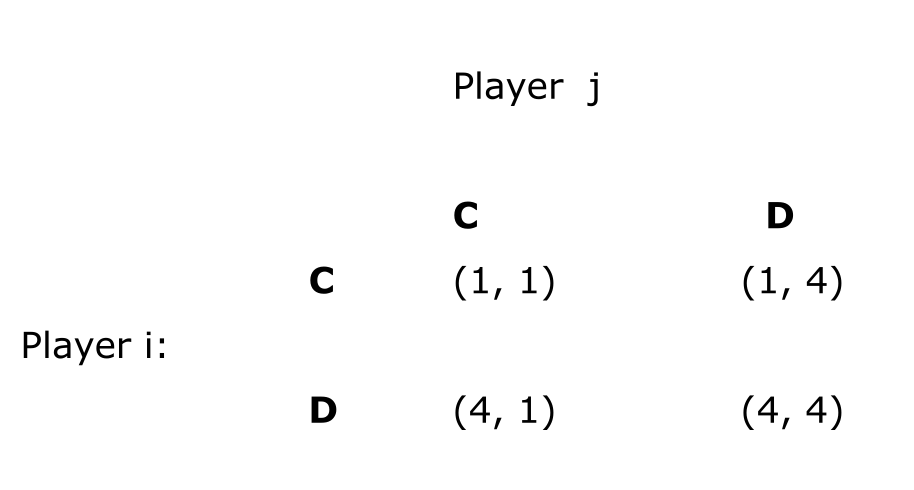
\includegraphics[width=\textwidth]{./images/rationalchoice.png}
    \caption{For player $j$, $D$ is the rational choice}
\end{figure}

\subsection{Dominant Strategy}
Given a particular strategy $s$ for agent $i$, there will be a number of possible outcomes.
We say $s_1$ dominates $s_2$ if every outcome possible by agent $i$ playing $s_1$ is preferred over every possible outcome by agent $i$ playing $s_2$.
A rational agent will never play a dominated strategy.
However, there is not usually a unique undominated strategy.

\subsection{Nash Equilibrium}
Two strategies $s_1$ and $s_2$ are in \textbf{Nash equilibrium} if:
\begin{itemize}
    \item   Assuming agent $i$ plays $s_1$, agent $j$ can do no better than play $s_2$; and
    \item   Assuming agent $j$ plays $s_2$, agent $i$ can do no better than play $s_1$.
\end{itemize}

In Nash equilibrium, neither agent has any incentive to deviate from their strategy.
Not all possible interactions have a Nash equilibrium, and some interactoins can have several Nash equilibria.

\subsection{Prisoner's Dilemma}
The \textbf{Prisoner's Dilemma} is usually expressed in terms of pay-offs (or rewards) for co-operating or defecting:

\[
\begin{array}{c c|c c}
  & & \text{Player } j & \\
  & & \text{C} & \text{D} \\
\hline
  \text{Player } i & \text{C} & (3, 3) & (0, 5) \\
                  & \text{D} & (5, 0) & (1, 1)
\end{array}
\]

\begin{itemize}
    \item   If both co-operate, they each get a reward of 3.
    \item   If both defect, they each get a reward of 1.
    \item   If one co-operates and the other defects, the com-operators gets 0 (the sucker's payoff) and the other gets 5.
\end{itemize}

The individually rational action is to defect:
it guarantees a payoff of no worse than 1, whereas co-operating guarantees a payoff of no worse than 0.
So, defection is the best response to all strategies;
however, common sense indicates that this is not the best response.
\\\\
The prisoner's dilemma occurs in many domains and is suitable for modelling large classes of multi-agent interactions.
There have been many real-world scenarios that are implicitly prisoner's dilemmas (or variations):
\begin{itemize}
    \item   Arms race;
    \item   Environmental issues;
    \item   Free-rider systems;
    \item   Warfare;
    \item   Behaviour in many biological systems --- bats, guppie fish, etc;
    \item   Competition between nodes in a distributed computer system;
    \item   Modelling competition and collaboration between information providers;
    \item   Sports.
\end{itemize}

Variations on the prisoner's dilemma include:
\begin{itemize}
    \item   \textbf{$N$-player dilemma:} for example, the voter's paradox, where it is true that a particular endeavour would return a benefit to all members where each individual would receive rewards;
            it is also true that any member would receive an even greater reward by contributing nothing.
            Elections, environment actions, and the tragedy of the commons are all examples of this phenomenon.

    \item   \textbf{Spatial organisations:} where agents are placed in some 2-dimensional space and can only interact with neighbours.

    \item   \textbf{Partial co-operation:} acts are no longer co-operative or non-co-operative, but can be in some range.
            If we consider extending the classical IPD to this domain, we can define landscapes using pay-off equations.

    \item   \textbf{Noise:} problems arise if we introduce any degree of noise, which will lead co-operations to be interpreted as defections, etc.
            Consider two TFTs playing witha  degree of noise.
\end{itemize}

Summay so far:
\begin{itemize}
    \item   We need a means to organise \& co-ordinate agents.
            There are underlying problems here with respect to co-operation.

    \item   Game theory \& extensions provides a tool to reason about and to develop multi-agent systems.

    \item   We assume agents have a rational ordering of possible outcomes and a set of actions they may choose to bring about those outcomes.

    \item   We have limited the types of interactions to very simple cases.
\end{itemize}

One extension is the \textbf{ultimatum game}.
We are no longer just discussing outcomes for simple choices:
\begin{itemize}
    \item   Two players $i$ and $j$.
    \item   The goal is to distribute some resource, e.g., €100.
    \item   Player $i$ picks a number $x$, in a range (0-100).
    \item   Player $j$ must accept or reject the offer.
    \item   If Player $j$ rejects: both get 0.
    \item   If Player $j$ accepts: Player $i$ gets $x$ and Player $j$ gets $100-x$.
\end{itemize}

This allows us to reason about more complex scenarios.
Many extensions are available and have been researched.
If we wish to reason about two or more agents/systems agreeing on value for some exchange (information, service), we can look to auction theory.
To reason about more complex scenarios, negotiation \& argumentation theory has been adopted.

\subsection{Auction Theory}
\textbf{Auction theory} can be used as a method to allow agents to arrive at an agreement regarding events \& actions when agents are self-interested.
In some cases, no agreement is possible at all.
However, in most scenarios, there is the potential to arrive at a mutually beneficial agreement.
There are several approaches that have been adopted to do this;
all can bee seen as a form of negotiation or argumentation by the agents.
Negotiation or argumentation is governed by some protocol or mechanism:
this protocol defines how the agents are to interact, i.e., the actual rules of encounter.
Questions that arise include:
\begin{itemize}
    \item   How to design a protocol such that certain properties exist?
    \item   How to design strategies for agents to use a given set of protocols?
\end{itemize}

Desired features from protocols include: guaranteed success, simplicity, maximising social utility, pareto-efficiency, \& individual rationality.
\textbf{Auctions} represent a class of useful protocols, and are used in many domains.
An auction takes place between an agent (auctioneer) and a set of other agents (bidders).
The goal is to allocate the goods to one of the bidders.
Usually, an auctioneer attempt to maximise the price;
the bidders desire to minimise the price.
We can categorise auctions according to a range of features:
\begin{itemize}
    \item   Bids may be:
            \begin{itemize}
                \item   Open-cry;
                \item   Sealed bid.
            \end{itemize}

    \item   Bidding may be:
            \begin{itemize}
                \item   One shot;
                \item   Ascending;
                \item   Descending.
            \end{itemize}
\end{itemize}

Selling goods by auction is more flexible than setting a fixed price and less time-consuming than explicit negotiation (haggling).
In many domains, the value of an item may vary enough to preclude direct \& absolute pricing.
It is a pure form of market;
it is efficient in that auctions usually ensure goods are allocated to those who value them most.
The price is set, not by the sellers, but by the buyers.
No one auction protocol is the best;
some are preferred by sellers, others by buyers.
Some auctions attempt to prevent cheating, or at least decrease the incentive to cheat;
others provide several means to cheat.
People tend to bid in auctions for two reasons:
\begin{itemize}
    \item   They wish to acquire the goods (bases bid on private evaluation).
    \item   They wish to acquire the goods to re-sell (bases bid on private evaluation and estimates on future valuations).
\end{itemize}

\subsubsection{English Auction}
In an \textbf{English auction}, the auctioneer begins with the lowest acceptable price (reserve), and proceeds to obtain successively higher bids from bidders until no-one will increase the bid.
It is effectively first-price, open-cry, \& ascending.
The dominant strategy is to successively bid a small amount more than the current highest id until it reaches their valuation, then withdraw.
Potential problems with English auctions include:
\begin{itemize}
    \item   Rings;
    \item   Shills in the bidders;
    \item   Winner's curse.
\end{itemize}

In some English auctions, the reserve price is kept secret to attempt to prevent rings from forming.

\subsubsection{Dutch Auction}
In a \textbf{Dutch auction}, bidding starts at an artificially high price.
Lower prices are offered, in descending order, until a bidder equals to the current price.
Goods are then sold to the bidder for that price
Dutch auctions are descending, open-cry auctions.
From a seller's perspective, the key to a successful auction is the effect of competition on the bidders.
In an English auction, a winner may pay well under their valuation and thus the seller loses out;
this is not the case in a Dutch auction.

\subsubsection{First-Price, Sealed Bid}
\textbf{First-price, sealed bid} auctions are usually one-shot auctions.
Each bidders submits a sealed bid.
The goods are sold to the highest bidders.
Best strategy is to bid to true valuation.
Interesting variations exist if there are a number of goods to be sold and a number of rounds.

\subsubsection{Vickrey Auction}
A \textbf{Vickrey auction} is a sealed-bid, second-price auction.
The price paid by the winner is that price offered by the second-placed bidder.
In this type of auction, contrary to initial intuition, sellers make as much, if not more than the first-price auctoins.
In reality, bidders are not afraid to bid high, knowing that they will have to pay the second price;
bidders tend to be more competitive.
\\\\
Other auction types exist also: reverse auctions, double auctions, haphazard (whisper auction, handshake auction), etc.
We can use auctions as a means to allow agents to agree on a price for buying goods or services.
Depending on the type of auction chosen, we will favour buyers or sellers.
We sill have some problems though:
\begin{itemize}
    \item   Are auctions the best way?
    \item   What happens following an auction, if upon receiving goods, one doesn't pay?
    \item   What happens following an auction, if upon paying, one realise that the goods are not as expected?
    \item   Is it possible to prevent shills, rings, \& other forms of manipulation?
    \item   In auctions, agents agree on a price; can we deal with more dimensions of negotiation?
\end{itemize}

\section{Automated Negotiation}
\textbf{Negotiation} is a means for a group to arrive at an agreement.
It is a process of joint decision-making where parties with different preferences seek to reach a mutually acceptable solution.
It is a fundamental mechanism in multi-agent systems \& human society.
Negotiation research deals with three topics:
\begin{itemize}
    \item   Negotiation protocols;
    \item   Negotiation objects; \&
    \item   Agents' decision-making models.
\end{itemize}

\subsection{Negotiation Protocols}
\textbf{Negotiation protocols} are a set of rules that govern the interaction:
\begin{itemize}
    \item   Includes the permitted type of participants;
    \item   Negotiation states;
    \item   Events that change states;
    \item   Actions of participants;
    \item   Rules for agreement formation; \&
    \item   Termination conditions.
\end{itemize}

\subsection{Negotiation Objects}
\textbf{Negotiation objects} consist of a range of issues over which agreement must be reached.
Related issues include the type of operations on agreements and altering the structure of the negotiation. 

\subsection{Agents' Decision-Making Models}
The \textbf{agents' decision-making models} are influenced by protocol, the nature of the negotiation objects, \& the range of operations.
The relative importance of the components varies depending on the domain.

\subsection{Domain Variation in Negotiation}
In some domains, the negotiation protocol is the dominant concern.
For example, in some auction settings, the best strategy for an agent is to bid to their true evaluation --- hence no strategic analysis is really required.
In other domains, the converse is true;
given the wide range of possibilities, there is no best technique for automated negotiation.

\subsection{Negotiation as Distributed Search}
Negotiation can be viewed as a \textbf{distributed search} through a space of potential agreements;
the dimensionality \& topology of this space is determined by the structure of the negotiation object.
One could consider each attribute of the negotiation object to have a separate dimension associated with it.
As dimensions are added (or removed), the number of points of agreement may increase (or decrease).
Similarly, if an agent changes one of the values, it is moving from one point in the agreement space to another.
\\\\
In a negotiation, participants are the active components that determine the direction of the search.
Initially, each agent will have a portion of the space in which it will be willing to make an agreement.
Also, agents will have some means to rate the points in the space.
Negotiation involves the agents suggesting points or spaces.

\subsection{Minimal Negotiation Capabilities}
The \textbf{minimal negotiation capabilities} are:
\begin{itemize}
    \item   To propose some point of space as being acceptable; \& 
    \item   To respond to such a proposal by indicating whether or not it is acceptable.
\end{itemize}

A simple setting is a Dutch auction:
\begin{itemize}
    \item   One agent (the auctioneer) calls out prices.
    \item   If there is no signal of acceptance by an agent, then the auctioneer makes a new offer which it believes will be more acceptable.
    \item   The process repeats.
\end{itemize}

If agents can only accept or reject offers, the negotiation will be very time-consuming \& inefficient.
The proposer is effectively picking points in the agreement space based on what it perceives \& hopes to stumble upon correct point. 
For negotiation to be more efficient, the recipient needs to offer feedback.

\subsection{Feedback in Negotiation}
\textbf{Feedback} can be a critique, or a counter-proposal.
A \textbf{critique} provides two forms of feedback:
it suggests constraints on issues, and indicates acceptation or rejection of particular negotiation issues.
The more information placed in the critique, the easier it is for the original agent to determine the boundaries of the agreement space.
\\\\
A \textbf{counter-proposal} is a proposal that is more favourable to the sender, made in response to a previous proposal.
It can suggest amendments or additions, provides implicit information about preferences, and can significantly speed up the negotiation process.

\subsection{Limitations of Simple Proposals}
Proposals, critiques, \& counter-proposals are mere statements of what the agents want; hence, the scope is confined.
Agents can't justify their negotiation stance or persuade one another to change the negotiation stance.
This leads to the idea of \textbf{argumentation-based negotiation}: allow agents to offer more information than available proposals, critiques, \& counter-proposals.

\subsection{Approaches to Negotiation}
Approaches to reasoning in a negotiation setting can be loosely categorised as game-theoretic, heuristic, or argumentation-based.

\subsubsection{Game-Theoretic Approach}
The \textbf{game-theoretic approach} can be applied in two manners:
\begin{itemize}
    \item   Designing appropriate protocols that will govern agent's interactions; \&
    \item   Design of a particular agent's strategy.
\end{itemize}

Properties of the game-theoretic approach include:
\begin{itemize}
    \item   We usually assume that a rational agent will choose the best strategy;
    \item   Finding the best strategy can be computationally intractable; \&
    \item   Disadvantages include that it may be difficult to characterise agent's preferences with respect to all possible outcomes.
\end{itemize}

\subsubsection{Heuristic Approach}
The \textbf{heuristic approach} seeks to search the negotiation space in a non-exhaustive fashion.
It produces good solutions rather than optimal solutions.
Disadvantages of the heuristic approach include:
\begin{itemize}
    \item   Sub-optimality: it adopts an approximate notion of rationality and does not fully examine the negotiation space;
    \item   Models need extensive analysis true simulation; \&
    \item   It is usually difficult to predict behaviour.
\end{itemize}

\subsubsection{Argumentation-Based Approach}
In the \textbf{argumentation-based approach}, agents aim to persuade or change the opponent's ratings over the agreement space.
Additional information is provided in addition to proposals, etc., usually taking the form of:
\begin{itemize}
    \item   \textbf{Threats:} ``if you don't accept, I'll have to...'';
    \item   \textbf{Rewards:} ``if you accept this offer, in the future I'll...''; \&
    \item   \textbf{Appeals:} ``this is standard practice in our industry...''.
\end{itemize}

\subsection{Extended Topics in Negotiation}
\subsubsection{Learning in Negotiation}
Agents can adapt strategies based on past interactions.
Types of learning:
\begin{itemize}
    \item   Learning opponent's preferences;
    \item   Learning effective negotiation strategies; \&
    \item   Learning from past negotiation outcomes.
\end{itemize}

\subsubsection{Trust \& Reputation}
\textbf{Trust \& reputation} are critical when agreements must be enforced overtime.
\textbf{Trust} models help agents to decide with whom to negotiate.
\textbf{Reputation} systems aggregate experiences across multiple agents.
There are mechanisms for:
\begin{itemize}
    \item   Preventing reneging on agreements;
    \item   Handling deception in negotiation; \&
    \item   Building long-term relationships.
\end{itemize}








\end{document}
